\documentclass[11pt,a4paper]{article}

\usepackage[UTF8]{ctex}
\usepackage[margin=1in]{geometry}
\usepackage{fontspec}
\setmainfont{Times New Roman}
\usepackage{enumitem}
\usepackage{hyperref}
\usepackage{xcolor}
\usepackage{titlesec}
\usepackage{graphicx}

\hypersetup{
  colorlinks=true,
  urlcolor=blue,
  linkcolor=blue,
  citecolor=blue
}

\titleformat{\section}{\large\bfseries}{}{0em}{}[\titlerule]
\titlespacing*{\section}{0pt}{8pt}{4pt}

\pagestyle{plain}
\setlength{\parindent}{0pt}
\setlist[itemize]{leftmargin=*,topsep=2pt,itemsep=1pt}

\begin{document}

\begin{center}
  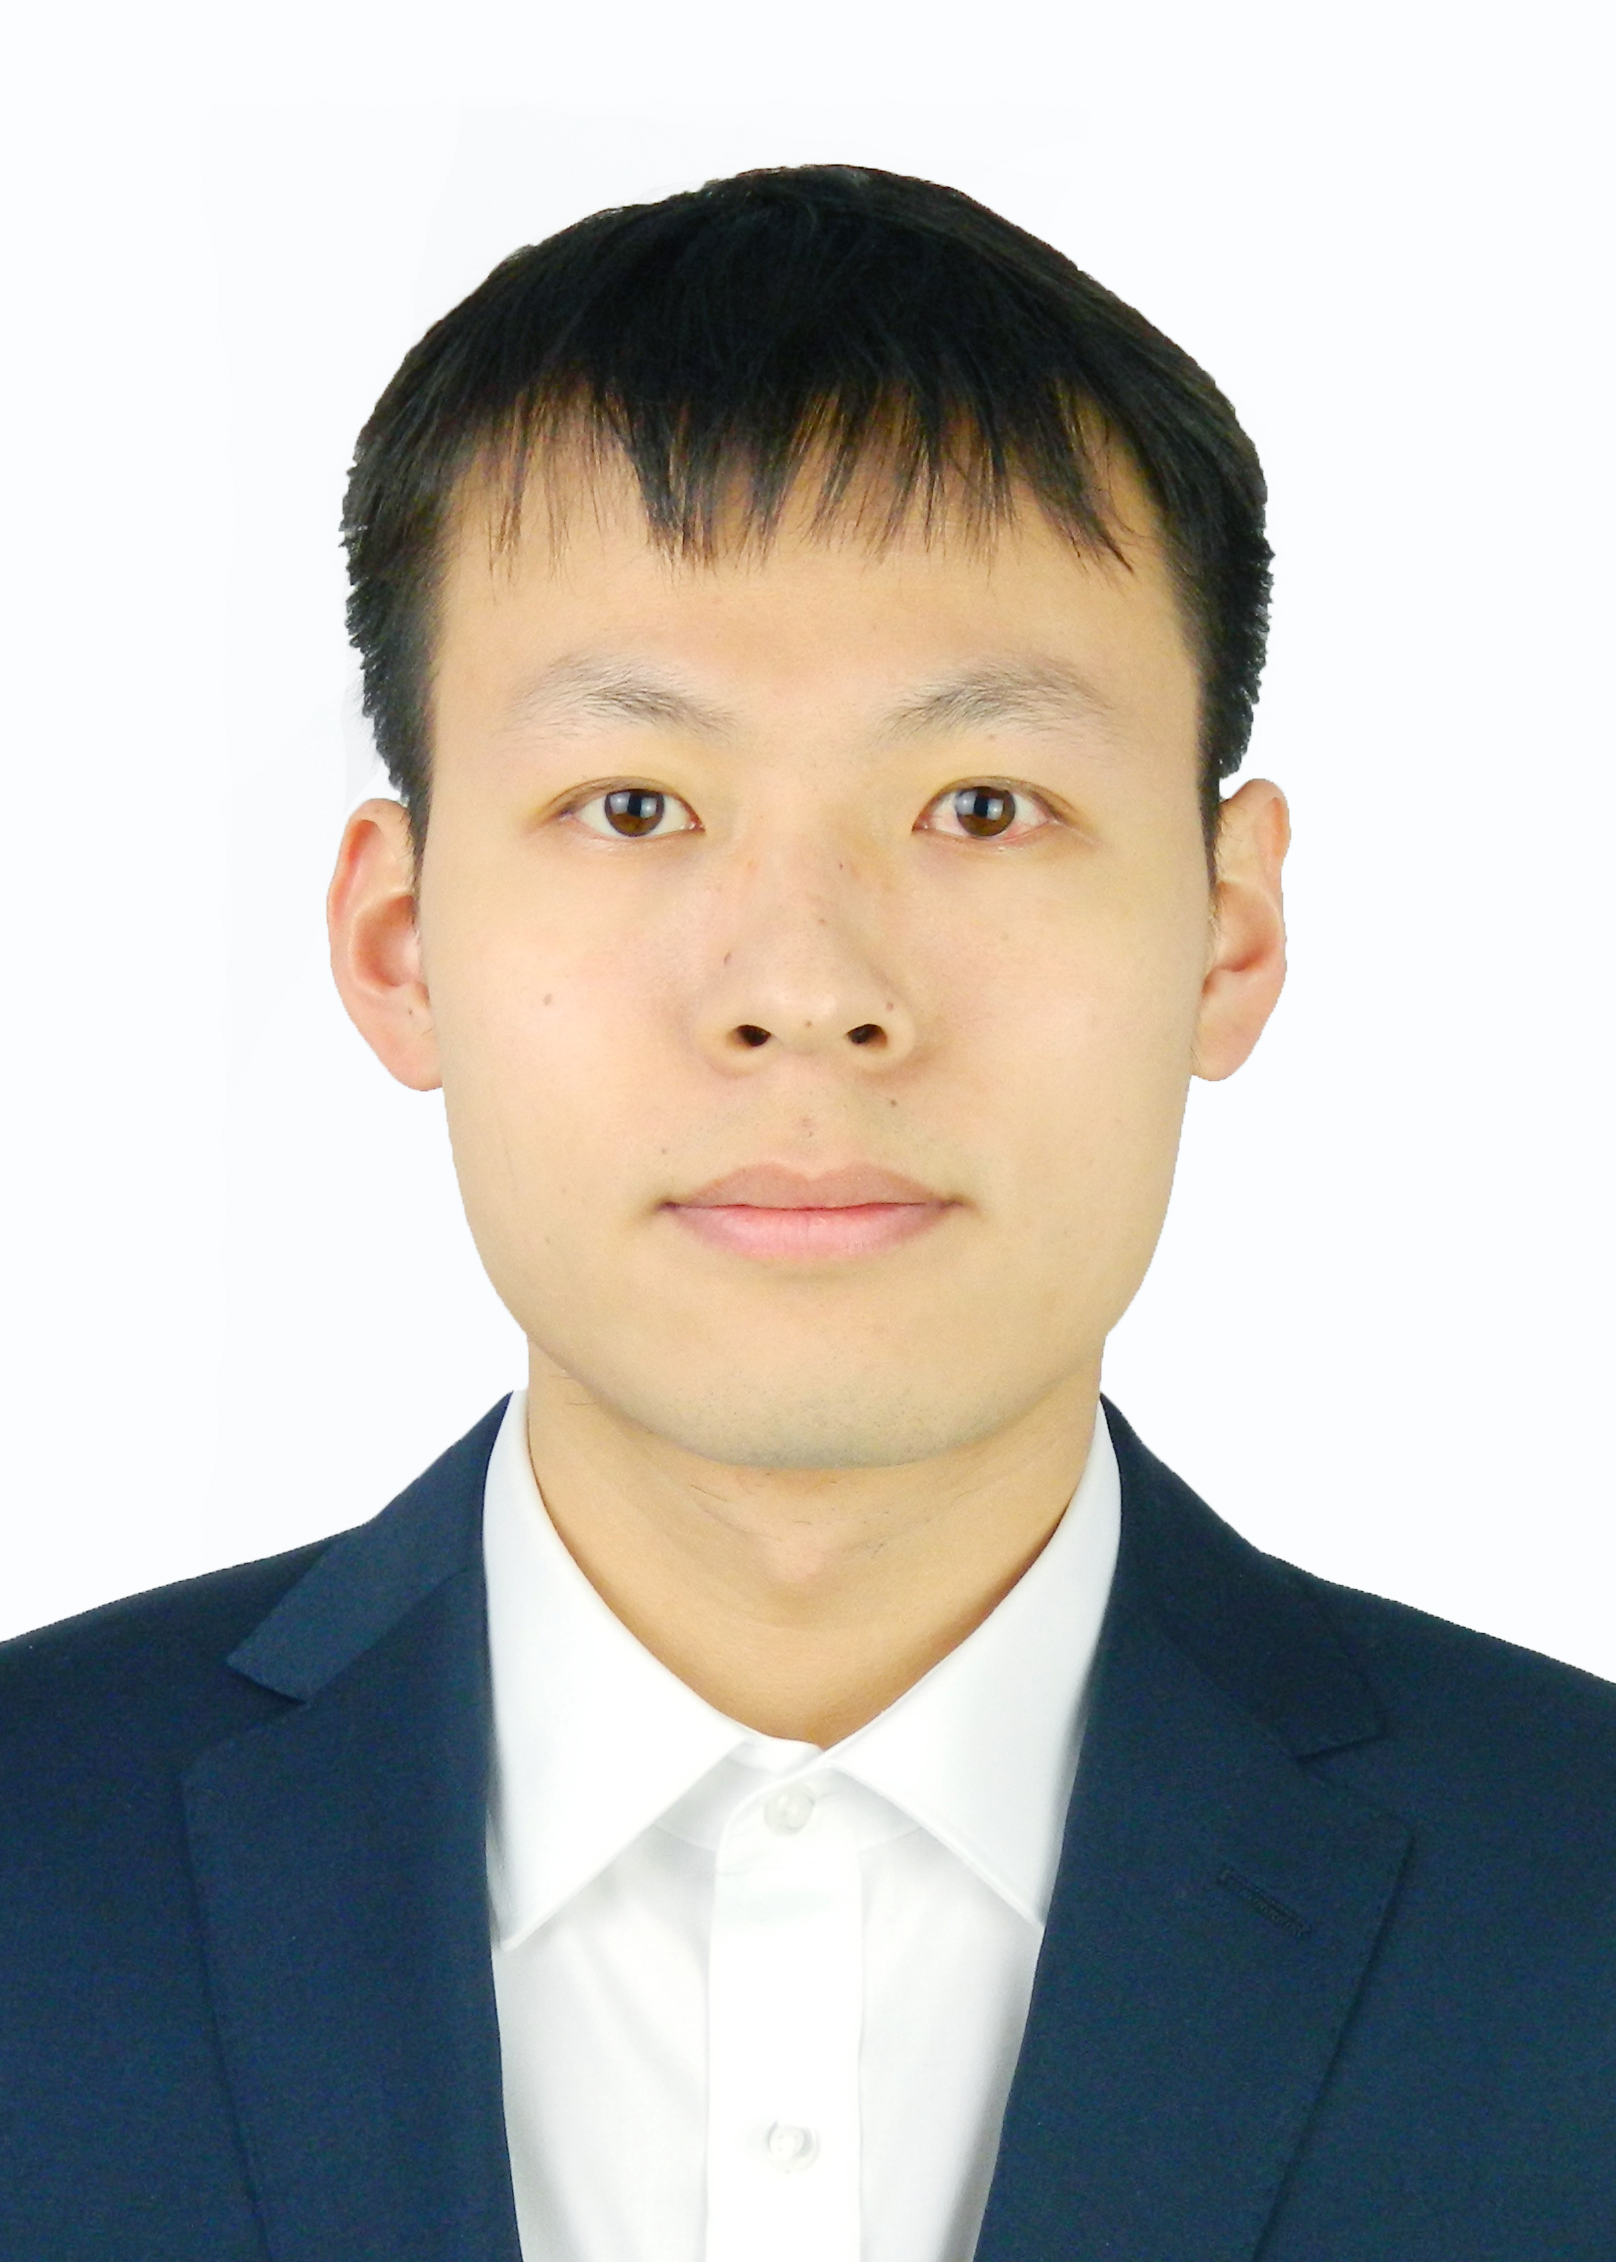
\includegraphics[width=2.5cm]{../zjc.jpg}\\[4pt]
  {\LARGE\bfseries Juchuan Zhang (张聚川)}\\[4pt]
  {\large Hardware Security Engineer, Huawei Technologies Co., Ltd.}\\[4pt]
  \href{mailto:juchuanzhang1994@gmail.com}{juchuanzhang1994@gmail.com}
  \quad | \quad
  \href{https://dblp.org/pid/220/2463.html}{DBLP}
  \quad | \quad
  \href{https://github.com/juchuanzhang}{GitHub}
  \quad | \quad
  \href{https://www.linkedin.com/in/\%E8\%81\%9A\%E5\%B7\%9D-\%E5\%BC\%A0-7337652a0/}{LinkedIn}
\end{center}

\vspace{6pt}

\section*{Research Interests}
Hardware Security, Microarchitecture Security, Side Channel Attacks

\section*{Education}
\textbf{Ph.D. in Control Theory and Control Engineering} \hfill 2017 -- 2022\\
Zhejiang University, USSLab\\
Advisor: Prof. Wenyuan Xu

\textbf{B.S. in Electrical Engineering and Automation} \hfill 2013 -- 2017\\
Xi'an Jiao Tong University

\section*{Experience}
\textbf{Hardware Security Engineer} \hfill 2022 -- Present\\
Huawei Technologies Co., Ltd.

\section*{Publications}

\subsection*{Journal Papers}
\begin{itemize}
  \item \textbf{[J4]} Yan Jiang, Xiaoyu Ji, \textbf{Juchuan Zhang}, Yancheng Jiang, Shui Jiang, Wenyuan Xu.
  ``CapSpeaker: Injecting Commands to Voice Assistants Via Capacitors.''
  \emph{IEEE Transactions on Dependable and Secure Computing (TDSC)}, 2024.

  \item \textbf{[J3]} Xiaoyu Ji, \textbf{Juchuan Zhang}, Shan Zou, Yi-Chao Chen, Gang Qu, Wenyuan Xu.
  ``MagView++: Data Exfiltration via CPU Magnetic Signals Under Video Decoding.''
  \emph{IEEE Transactions on Mobile Computing (TMC)}, 2024.

  \item \textbf{[J2]} Xiaoyu Ji, Yushi Cheng, \textbf{Juchuan Zhang}, Yuehan Chi, Wenyuan Xu, Yi-Chao Chen.
  ``Device Fingerprinting with Magnetic Induction Signals Radiated by CPU Modules.''
  \emph{ACM Transactions on Sensor Networks (TOSN)}, 2022.

  \item \textbf{[J1]} Xiaoyu Ji, Chaohao Li, Xinyan Zhou, \textbf{Juchuan Zhang}, Yanmiao Zhang, Wenyuan Xu.
  ``Authenticating Smart Home Devices via Home Limited Channels.''
  \emph{ACM Transactions on Internet of Things (TIOT)}, 2020.
\end{itemize}

\subsection*{Conference Papers}
\begin{itemize}
  \item \textbf{[C7]} Shan Zou, \textbf{Juchuan Zhang}, Shui Jiang, Yushi Cheng, Xiaoyu Ji, Wenyuan Xu.
  ``OutletGuarder: Detecting DarkSide Ransomware by Power Factor Correction Signals in an Electrical Outlet.''
  \emph{ICPADS}, 2022.

  \item \textbf{[C6]} Xiaoyu Ji, \textbf{Juchuan Zhang}, Shui Jiang, Jishen Li, Wenyuan Xu.
  ``CapSpeaker: Injecting Voices to Microphones via Capacitors.''
  \emph{ACM CCS}, 2021.

  \item \textbf{[C5]} \textbf{Juchuan Zhang}, Xiaoyu Ji, Yuehan Chi, Yi-Chao Chen, Bin Wang, Wenyuan Xu.
  ``OutletSpy: Cross-Outlet Application Inference via Power Factor Correction Signal.''
  \emph{ACM WiSec}, 2021.

  \item \textbf{[C4]} \textbf{Juchuan Zhang}, Xiaoyu Ji, Wenyuan Xu, Yi-Chao Chen, Yuting Tang, Gang Qu.
  ``MagView: A Distributed Magnetic Covert Channel via Video Encoding and Decoding.''
  \emph{IEEE INFOCOM}, 2020.

  \item \textbf{[C3]} Yushi Cheng, Xiaoyu Ji, \textbf{Juchuan Zhang}, Wenyuan Xu, Yi-Chao Chen.
  ``DeMiCPU: Device Fingerprinting with Magnetic Signals Radiated by CPU.''
  \emph{ACM CCS}, 2019.

  \item \textbf{[C2]} Chaohao Li, Xiaoyu Ji, Xinyan Zhou, \textbf{Juchuan Zhang}, Jing Tian, Yanmiao Zhang, Wenyuan Xu.
  ``HlcAuth: Key-free and Secure Communications via Home-Limited Channel.''
  \emph{ACM AsiaCCS}, 2018.

  \item \textbf{[C1]} Zhou Zhuang, Xiaoyu Ji, Taimin Zhang, \textbf{Juchuan Zhang}, Wenyuan Xu, Zhenhua Li, Yunhao Liu.
  ``FBSleuth: Fake Base Station Forensics via Radio Frequency Fingerprinting.''
  \emph{ACM AsiaCCS}, 2018.
\end{itemize}

\end{document}